\documentclass{article}
\usepackage{times}
\usepackage[hidelinks,bookmarks]{hyperref}
\usepackage{url}
\usepackage{tabularx}
\usepackage{graphicx}
\usepackage{placeins}

% configuration of source code examples
\usepackage{listings}
\lstset{language=verilog}
\lstset{numbers=left}
\lstset{xleftmargin=2em}
\lstset{framexleftmargin=2em}
\lstset{tabsize=4}
\lstset{frame=single}
\lstset{breaklines=true}
\lstset{showspaces=false}
\lstset{showstringspaces=false}
\lstset{showtabs=false}
\lstset{breakatwhitespace=false}

\setcounter{tocdepth}{2}

\begin{document}

\title{GreenPak4 HDL Place-And-Route User Guide}
\author{Andrew Zonenberg\\
azonenberg@drawersteak.com}
\date{\today}
\maketitle

\begin{abstract}
This document is the primary reference manual for gp4par, Andrew Zonenberg's place-and-route tool for Silego 
GreenPak4 devices. As of this writing, the toolchain is NOT officially supported or endorsed by Silego and not all 
GreenPak4 devices are supported. It is under active development and should be considered alpha quality.
\end{abstract}

\pagebreak

\tableofcontents

\pagebreak
\section{Revision History}
\begin{itemize}
\item \today: [in progress] Initial draft
\end{itemize}

\pagebreak
\section{Introduction}

\subsection{Architecture Support}
This guide will eventually apply to all Silego GreenPak4 devices. As of this writing the toolchain is still under early
development and only the SLG46620V is supported.

\subsection{Coding Examples}
The coding examples in this guide are accurate as of the date of publication. The most up-to-date version of this 
document, as well as source code for the place-and-route tool, may be found on GitHub at 
\url{https://github.com/azonenberg/openfpga/}.

\subsection{Syntax Examples}
The syntax examples in this guide show how to use constraints and options. The examples are comprehensive; only the 
described syntax for a particular constraint or option is guaranteed to work.

All Verilog attributes and values are case sensitive unless otherwise noted.

\subsection{Acronyms}

\begin{tabularx}{4in}{|l|X|}
\hline
{\bfseries Acronym} & {\bfseries Meaning} \\
\hline
HDL & Hardware Description Language \\
\hline
IOB & Input/Output Buffer \\
\hline
PAR & Place And Route \\
\hline
RTL & Register Transfer Level \\
\hline
\end{tabularx}

\pagebreak
\section{Synthesizing a Netlist}

\subsection{Design Flow}

gp4par is NOT a synthesis tool and cannot be run directly on HDL source code. Your HDL must be synthesized to
a JSON netlist by a separate tool before gp4par may be invoked. The recommended synthesis tool is 
\emph{yosys}, which may be obtained from the Yosys website (\url{http://www.clifford.at/yosys/}). The flow of data 
between components is shown in Figure. \ref{flow}.

\begin{figure}[h]
\centering
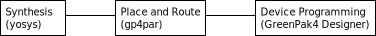
\includegraphics[scale=1]{figures/flow.pdf}
\caption{Data flow between toolchain components}
\label{flow}
\end{figure}

gp4par is being developed in tandem with GreenPak support in Yosys. Most of the GreenPak features are only available in 
the latest development version of Yosys and have not made it into a stable release yet. We recommend use of the latest 
Yosys from GitHub for testing.

\subsection{Synthesis Example}

A simple synthesis script for \emph{yosys} is shown in figure \ref{yscript}. The script synthesizes a single Verilog 
source file \texttt{Blinky.v}, with a top-level module \texttt{BlinkyTop}, to the netlist \texttt{Blinky.json} and 
targets the SLG46620V. This script is only a starting point and may be customized as needed. This document does not
cover synthesis commands; please see the online documentation for \emph{yosys} for command documentation.
\begin{figure}[h]
\begin{lstlisting}[language=sh]
#!/usr/bin/env yosys
read_verilog Blinky.v
synth_greenpak4 -top BlinkyTop -part SLG46620V -json /tmp/Blinky.json
\end{lstlisting}
\caption{Example synthesis script}
\label{yscript}
\end{figure}

\pagebreak
\section{gp4par Limitations}

The following legal Verilog-2001 features are not supported by gp4par as of this writing:

\begin{itemize}
\item {\bfseries Bidirectional or tri-state top-level module ports}\\All ports on top-level modules must be inputs, 
push-pull, or open-drain outputs. There is no support for tri-state or bidirectional outputs.
\item {\bfseries Non-scalar top-level module ports}\\All ports on top-level modules must be one bit wide. Vector nets 
may be used at lower levels of the hierarchy without restriction as long as the synthesis script includes a
``splitnets" command to convert these to single bit nets. (The synth\_greenpak4 Yosys command includes this command by 
default.)
\end{itemize}

The following SLG46620V device features are not supported by gp4par as of this writing:

\begin{itemize}
\item Storage elements: output inverter, latch mode
\item Counters: Delay, FSM, edge detector, PWM, wake-sleep mode, counter cascading.
All clock sources other than on-chip oscillator. Pre-divider value of 12.
\item Voltage reference: DAC, divided Vdd, external references
\item Comparators: Buffered input on pin 6, global buffer bandwidth selection, routing from PGA, speed doubler
\item PGA
\item ADC
\item DAC
\item PGEN mode of LUT4/PGEN block
\item Wake-Sleep
\item DCMP/PWM
\item Programmble delay line / edge detector
\item Slave SPI
\item Pin 8 reset output
\end{itemize}

\pagebreak
\section{gp4par HDL Constraints}

There is only one supported constraint entry format at this time, Verilog attributes. There is currently no support for 
adding constraints to netlist entities via external constraint files or command line arguments. The general format of a 
constraint with name \texttt{FOO} and value 42 applied to the register \texttt{foobar} is shown in Figure 
\ref{constraint}.

\begin{figure}[h]
\begin{lstlisting}
(* FOO=42 *)
reg[3:0] foobar = 0;
\end{lstlisting}
\caption{Example Verilog attribute constraint}
\label{constraint}
\end{figure}

%%%%%%%%%%%%%%%%%%%%%%%%%%%%%%%%%%%%%%%%%%%%%%%%%%%%%%%%%%%%%%%%%%%%%%%%%%%%%%%%%%%%%%%%%%%%%%%%%%%%%%%%%%%%%%%%%%%%%%%%
% COUNT_EXTRACT

\pagebreak
\subsection{Counter Extraction (COUNT\_EXTRACT)}
\label{count-extract}

The COUNT\_EXTRACT constraint controls inference of GP\_COUNT8 and GP\_COUNT14 cells from behavioral Verilog. It can be 
used to ensure that a given counter in behavioral logic will, or will not be, mapped to a hard macro.

\subsubsection{Applicable Elements}
The COUNT\_EXTRACT constraint may only be used on vector registers.

\subsubsection{Constraint Values}
\begin{itemize}
\item {\bfseries Vector register}\\
One of the following:
\begin{itemize}
\item AUTO: Same behavior as not specifying any constraint. Counters will be inferred where possible.
\item NO: Do not infer a counter even if the logic matches a supported inference structure.
\item FORCE: Always infer a counter. If a supported inference structure is not found, a synthesis error is produced.
\end{itemize}
\item {\bfseries Other} \\
This constraint will be silently ignored if used on any other entity.
\end{itemize}

\clearpage
\subsubsection{Verilog Usage Example}

Figure \ref{constraint-count-extract} is an example of a 5-bit down counter with a positive level triggered reset, 
configured to force counter inference.

\begin{figure}[h]
\begin{lstlisting}
(* COUNT_EXTRACT = "FORCE" *)
reg[4:0] count = COUNT_MAX;
wire out = (count == 0);
always @(posedge clk, posedge count_rst) begin
	
	//level triggered reset
	if(count_rst)
		count		<= 0;
	
	//counter
	else begin

		if(count == 0)
			count	<= COUNT_MAX;
		else
			count	<= count - 1'd1;

	end
	
end
\end{lstlisting}
\caption{Example for COUNT\_EXTRACT constraint}
\label{constraint-count-extract}
\end{figure}

%%%%%%%%%%%%%%%%%%%%%%%%%%%%%%%%%%%%%%%%%%%%%%%%%%%%%%%%%%%%%%%%%%%%%%%%%%%%%%%%%%%%%%%%%%%%%%%%%%%%%%%%%%%%%%%%%%%%%%%%
% Drive type

\pagebreak
\subsection{Drive Type (DRIVE\_TYPE)}

The DRIVE\_TYPE constraint configures the output driver on the specified I/O pin.

\subsubsection{Applicable Elements}
The DRIVE\_TYPE constraint may only be used on top-level module ports. 

\subsubsection{Constraint Values}
\begin{itemize}
\item {\bfseries Top-level module port (IOB)}
	\begin{itemize}
		\item ``NMOS\_OD": Open drain NMOS pull-down driver.
		\item ``PMOS\_OD": Open drain PMOS pull-down driver.
		\item ``PUSHPULL": CMOS digital push-pull driver. This is the default if no constraint is specified..
	\end{itemize}
\item {\bfseries Other} \\
This constraint may not be used on any other entity.
\end{itemize}

\subsubsection{Verilog Usage Example}

Figure \ref{constraint-drivetype} is an example of a top-level module with two ports \texttt{a} and \texttt{b}. Port 
\texttt{a} has a push-pull driver and port \texttt{b} has an open-drain NMOS driver.

\begin{figure}[h]
\begin{lstlisting}
module Foo(a, b);

	(* DRIVE_TYPE = "PUSHPULL" *)
	output wire a;

	(* DRIVE_TYPE = "NMOS_OD" *)
	output wire b;
	
endmodule
\end{lstlisting}
\caption{Example for DRIVE\_TYPE constraint}
\label{constraint-drivetype}
\end{figure}

%%%%%%%%%%%%%%%%%%%%%%%%%%%%%%%%%%%%%%%%%%%%%%%%%%%%%%%%%%%%%%%%%%%%%%%%%%%%%%%%%%%%%%%%%%%%%%%%%%%%%%%%%%%%%%%%%%%%%%%%
% Input buffer type

\pagebreak
\subsection{Input Buffer Type (IBUF\_TYPE)}

The IBUF\_TYPE constraint configures the input buffer on the specified I/O pin.

\subsubsection{Applicable Elements}
The IBUF\_TYPE constraint may only be used on top-level module ports. 

\subsubsection{Constraint Values}
\begin{itemize}
\item {\bfseries Top-level module port (IOB)}
	\begin{itemize}
		\item ``ANALOG": Analog buffer for mixed signal IP. Analog outputs must use this setting to disable the digital 
		input buffer.
		\item ``LOW\_VOLTAGE": Low voltage threshold (see datasheet for exact value)
		\item ``NORMAL": Standard threshold (see datasheet for exact value(
	\end{itemize}
\item {\bfseries Other} \\
This constraint may not be used on any other entity.
\end{itemize}

\subsubsection{Verilog Usage Example}

Figure \ref{constraint-ibuftype} FIXME

\begin{figure}[h]
\begin{lstlisting}
\end{lstlisting}
\caption{Example for IBUF\_TYPE constraint}
\label{constraint-ibuftype}
\end{figure}

%%%%%%%%%%%%%%%%%%%%%%%%%%%%%%%%%%%%%%%%%%%%%%%%%%%%%%%%%%%%%%%%%%%%%%%%%%%%%%%%%%%%%%%%%%%%%%%%%%%%%%%%%%%%%%%%%%%%%%%%
% LOC

\pagebreak
\subsection{Physical Location (LOC)}

The LOC constraint instructs gp4par to place the constrained net or primitive at a specific physical site of the 
device.

\subsubsection{Applicable Elements}
As of this writing, the LOC constraint may only be used on top-level module ports. 

\subsubsection{Constraint Values}
\begin{itemize}
\item {\bfseries Top-level module port}\\
Text string ``Pn" where \texttt{n} is the pin number of the device. Example: ``P3", ``P17".
\item {\bfseries Other} \\
This constraint may not be used on any other entity. Future versions of gp4par may allow use of this constraint 
to lock LUTs, flipflops, and hard IP to specific locations.
\end{itemize}

\subsubsection{Verilog Usage Example}

Figure \ref{constraint-loc} is an example of a top-level module with three ports \texttt{a}, \texttt{b}, and \texttt{o}.
These ports are constrained to package pins 20, 19, and 18 respectively.

\begin{figure}[h]
\begin{lstlisting}
module Foo(a, b, o);

	(* LOC = "P20" *)
	input wire a;

	(* LOC = "P19" *)
	input wire b;

	(* LOC = "P18" *)
	output wire o;
	
endmodule
\end{lstlisting}
\caption{Example for LOC constraint}
\label{constraint-loc}
\end{figure}

%%%%%%%%%%%%%%%%%%%%%%%%%%%%%%%%%%%%%%%%%%%%%%%%%%%%%%%%%%%%%%%%%%%%%%%%%%%%%%%%%%%%%%%%%%%%%%%%%%%%%%%%%%%%%%%%%%%%%%%%
% Pulldown

\pagebreak
\subsection{Pull-Down Resistor (PULLDOWN)}

The PULLDOWN constraint instructs gp4par to enable the pull-down resistor on the specified input. The exact resistor 
value ranges may be found in the device datasheet.

\subsubsection{Applicable Elements}
The PULLDOWN constraint may only be used on top-level module ports. 

\subsubsection{Constraint Values}
\begin{itemize}
\item {\bfseries Top-level module port (IOB)}\\
Text string ``10k", ``100k", or ``1M", case sensitive, to specify the nominal value of the pull-down resistor.
\item {\bfseries Other} \\
This constraint may not be used on any other entity.
\end{itemize}

\subsubsection{Verilog Usage Example}

Figure \ref{constraint-pulldown} is an example of a top-level module with three ports \texttt{a}, \texttt{b}, and
\texttt{o}. Ports \texttt{a} and \texttt{b} have 10k$\Omega$ pull-down resistors; port \texttt{o} is floating.

\begin{figure}[h]
\begin{lstlisting}
module Foo(a, b, o);

	(* PULLDOWN = "10k" *)
	input wire a;

	(* PULLDOWN = "10k" *)
	input wire b;

	input wire o;
	
endmodule
\end{lstlisting}
\caption{Example for PULLDOWN constraint}
\label{constraint-pulldown}
\end{figure}

%%%%%%%%%%%%%%%%%%%%%%%%%%%%%%%%%%%%%%%%%%%%%%%%%%%%%%%%%%%%%%%%%%%%%%%%%%%%%%%%%%%%%%%%%%%%%%%%%%%%%%%%%%%%%%%%%%%%%%%%
% Pullup

\pagebreak
\subsection{Pull-Up Resistor (PULLUP)}

The PULLUP constraint instructs gp4par to enable the pull-up resistor on the specified input. The exact resistor 
value ranges may be found in the device datasheet.

\subsubsection{Applicable Elements}
The PULLUP constraint may only be used on top-level module ports. 

\subsubsection{Constraint Values}
\begin{itemize}
\item {\bfseries Top-level module port (IOB)}\\
Text string ``10k", ``100k", or ``1M", case sensitive, to specify the nominal value of the pull-up resistor.
\item {\bfseries Other} \\
This constraint may not be used on any other entity.
\end{itemize}

\subsubsection{Verilog Usage Example}

Figure \ref{constraint-pullup} is an example of a top-level module with three ports \texttt{a}, \texttt{b}, and
\texttt{o}. Ports \texttt{a} and \texttt{b} have 10k$\Omega$ pull-up resistors; port \texttt{o} is floating.

\begin{figure}[h]
\begin{lstlisting}
module Foo(a, b, o);

	(* PULLUP = "10k" *)
	input wire a;

	(* PULLUP = "10k" *)
	input wire b;

	input wire o;
	
endmodule
\end{lstlisting}
\caption{Example for PULLUP constraint}
\label{constraint-pullup}
\end{figure}

%%%%%%%%%%%%%%%%%%%%%%%%%%%%%%%%%%%%%%%%%%%%%%%%%%%%%%%%%%%%%%%%%%%%%%%%%%%%%%%%%%%%%%%%%%%%%%%%%%%%%%%%%%%%%%%%%%%%%%%%
% Schmitt Trigger

\pagebreak
\subsection{Schmitt Trigger (SCHMITT\_TRIGGER)}

The SCHMITT\_TRIGGER constraint instructs gp4par to enable the Schmitt trigger on the specified input. The level 
of hysterisis provided may be found in the device datasheet.

\subsubsection{Applicable Elements}
The SCHMITT\_TRIGGER constraint may only be used on top-level module ports configured in bidirectional or input mode. 

\subsubsection{Constraint Values}
\begin{itemize}
\item {\bfseries Top-level module port (IOB)}\\
Any nonzero value, or no value, to enable the Schmitt trigger. Specify zero, or no constraint, to disable it.
\item {\bfseries Other} \\
This constraint may not be used on any other entity.
\end{itemize}

\subsubsection{Verilog Usage Example}

Figure \ref{constraint-schmitt} is an example of a top-level module with three ports \texttt{a}, \texttt{b}, and
\texttt{o}. The Schmitt trigger is enabled for ports  \texttt{a} and \texttt{b}, but not \texttt{o}.

\begin{figure}[h]
\begin{lstlisting}
module Foo(a, b, o);

	(* SCHMITT_TRIGGER = 1 *)
	input wire a;

	(* SCHMITT_TRIGGER *)
	input wire b;

	(* SCHMITT_TRIGGER = 0 *)
	input wire o;
	
endmodule
\end{lstlisting}
\caption{Example for SCHMITT\_TRIGGER constraint}
\label{constraint-schmitt}
\end{figure}

%%%%%%%%%%%%%%%%%%%%%%%%%%%%%%%%%%%%%%%%%%%%%%%%%%%%%%%%%%%%%%%%%%%%%%%%%%%%%%%%%%%%%%%%%%%%%%%%%%%%%%%%%%%%%%%%%%%%%%%%
% SHREG_EXTRACT

\pagebreak
\subsection{Shift Register Extraction (SHREG\_EXTRACT)}
\label{shreg-extract}

The SHREG\_EXTRACT constraint controls inference of GP\_SHREG cells from behavioral Verilog. It can be 
used to ensure that a given shift register in behavioral logic will, or will not be, mapped to a hard macro.

\subsubsection{Applicable Elements}
The SHREG\_EXTRACT constraint may only be used on 1-bit registers.

\subsubsection{Constraint Values}
\begin{itemize}
\item {\bfseries Single-bit register}\\
One of the following:
\begin{itemize}
\item AUTO: Same behavior as not specifying any constraint. Shift registers will be inferred where possible.
\item NO: Do not infer a shift register even if the logic matches a supported inference structure.
\item FORCE: Always infer a shift register. If a supported inference structure is not found, a synthesis error is produced.
\end{itemize}
\item {\bfseries Other} \\
This constraint will be silently ignored if used on any other entity.
\end{itemize}

\clearpage
\subsubsection{Verilog Usage Example}

Figure \ref{constraint-shreg-extract} is an example of FIXME

\begin{figure}[h]
\begin{lstlisting}
FIXME
\end{lstlisting}
\caption{Example for SHREG\_EXTRACT constraint}
\label{constraint-shreg-extract}
\end{figure}

%%%%%%%%%%%%%%%%%%%%%%%%%%%%%%%%%%%%%%%%%%%%%%%%%%%%%%%%%%%%%%%%%%%%%%%%%%%%%%%%%%%%%%%%%%%%%%%%%%%%%%%%%%%%%%%%%%%%%%%%
% Timing constraints

\pagebreak
\section{gp4par Timing Constraints}

Static timing analysis is not yet implemented, thus this section is currently blank.

%%%%%%%%%%%%%%%%%%%%%%%%%%%%%%%%%%%%%%%%%%%%%%%%%%%%%%%%%%%%%%%%%%%%%%%%%%%%%%%%%%%%%%%%%%%%%%%%%%%%%%%%%%%%%%%%%%%%%%%%
% Coding Techniques

\pagebreak
\section{gp4par HDL Coding Techniques}

When possible, we recommend inferring design elements to maximize design portability. In some cases, such as for hard 
IP blocks or when exact control over synthesis results is required, it may be necessary to manually instantiate device 
primitives.

%%%%%%%%%%%%%%%%%%%%%%%%%%%%%%%%%%%%%%%%%%%%%%%%%%%%%%%%%%%%%%%%%%%%%%%%%%%%%%%%%%%%%%%%%%%%%%%%%%%%%%%%%%%%%%%%%%%%%%%%
% Counters

\subsection{Counters}

Yosys provides limited inference capability for counters which match the capabilities of the hard macro counters 
(GP\_COUNT8 and GP\_COUNT14) in the device.

Some hard macro capabilities (most notably input dividers) are not yet supported for inference; if these capabilities 
are required then use explicit primitive instantiation. Future software releases will expand the set of counter 
features which may be inferred.

\subsubsection{Inference Requirements}

In order to be inferred, a counter must:

\begin{itemize}
\item Be less than 14 bits in width
\item Count down only
\item Be initialized to the same (maximum) value by both underflow and by power-on reset
\item Have either no reset, or a positive level triggered reset to zero
\item Not have any logic use the internal counter register. Only the ``underflow" signal may be used by surrounding logic.
\end{itemize}

\subsubsection{Counter Related Constraints}

By default, the ``greenpak4\_counters" pass will attempt to infer a counter macro for every counter matching the 
requirements. If this is not desired, use the COUNT\_EXTRACT constraint (Section \ref{count-extract}) to control 
inference behavior.

\clearpage
\subsubsection{Verilog Usage Example}

The example in Figure \ref{gp-countinfer-example} shows an example of how to infer a resettable down counter.

\begin{figure}[h]
\begin{lstlisting}
localparam COUNT_MAX = 31;
reg[4:0] count = COUNT_MAX;
wire underflow_out = (count == 0);
always @(posedge clk, posedge count_rst) begin
	
	if(count_rst)
		count			<= 0;
	
	else begin

		if(count == 0)
			count		<= COUNT_MAX;
		else
			count		<= count - 1'd1;

	end
	
end
\end{lstlisting}
\caption{Example for counter inference}
\label{gp-countinfer-example}
\end{figure}

\subsubsection{Reporting}

In order to determine whether a given counter was extracted, look at the synthesis report. Figure 
\ref{counter-extraction} shows an example synthesis report with a single inferred counter.

\begin{figure}[h]
{\small
\begin{verbatim}
2.7.
Executing GREENPAK4_COUNTERS pass (mapping counters to hard IP blocks).
  Found 3-bit non-resettable down counter (from 7) for register count
    declared at Blinky.v:93
Extracted 1 counters
\end{verbatim}
}
\caption{Sample extraction report}
\label{counter-extraction}
\end{figure}

%%%%%%%%%%%%%%%%%%%%%%%%%%%%%%%%%%%%%%%%%%%%%%%%%%%%%%%%%%%%%%%%%%%%%%%%%%%%%%%%%%%%%%%%%%%%%%%%%%%%%%%%%%%%%%%%%%%%%%%%
% Shift Registers

\pagebreak
\subsection{Shift Registers}

Yosys provides inference capability for shift registers matching the capabilities of the ``pipe delay" block in the 
SLG46620/21.

The internal inverter is not yet supported for inference. If this is required for your design, consider manual 
instantiation of a GP\_SHREG primitive.

\subsubsection{Inference Requirements}

In order to be inferred as a single GP\_SHREG primitive, a shift register must:

\begin{itemize}
\item Be at most 16 bits in depth
\item Be initialized to zero (FIXME: confirm with Silego)
\item Have either no reset, or a positive level triggered reset to zero
\item Have at most two taps in the shift register connected to external logic. If more taps are required, a second 
shift register and/or discrete flipflops may be inferred. 
\end{itemize}

\subsubsection{Shift Register Related Constraints}

As of now there are no constraints to force or disable inference of shift registers. A constraint analogous to 
COUNT\_EXTRACT will likely be added in a future software release.

\clearpage
\subsubsection{Verilog Usage Example}

The example in Figure \ref{gp-shreginfer-example} shows an example of how to infer a shift register with taps delayed 8 
and 16 clocks from the input.

\begin{figure}[h]
\begin{lstlisting}
wire led_in;
reg[15:0] led_shreg = 0;
assign led1 = led_shreg[7];
assign led2 = led_shreg[15];
always @(posedge clk) begin
	led_shreg	<= {led_shreg[14:0], led_in};
end
\end{lstlisting}
\caption{Example for shift register inference}
\label{gp-shreginfer-example}
\end{figure}

\subsubsection{Reporting}

In order to determine whether a given shift register was extracted, look at the synthesis report. Figure 
\ref{shreg-extraction} shows an example synthesis report with a single inferred shift register.

\begin{figure}[h]
{\small
\begin{verbatim}
2.15. Executing SHREGMAP pass (map shift registers).
Converting Blinky.$auto$simplemap.cc:373:simplemap_dff$132 ...
  Blinky.$auto$simplemap.cc:373:simplemap_dff$147 to a shift
  register with depth 16.
Converted 16 dff cells into 1 shift registers.
\end{verbatim}
}
\caption{Sample extraction report}
\label{shreg-extraction}
\end{figure}

%%%%%%%%%%%%%%%%%%%%%%%%%%%%%%%%%%%%%%%%%%%%%%%%%%%%%%%%%%%%%%%%%%%%%%%%%%%%%%%%%%%%%%%%%%%%%%%%%%%%%%%%%%%%%%%%%%%%%%%%
% Primitives

\pagebreak
\section{gp4par Verilog Primitives}

This section lists all of the device-dependent primitives wrapping hard IP blocks in the device. These may be used for 
features which are not yet supported by inference, or when exact control over synthesis results is needed.

Pay careful attention to port names and descriptions as these may not exactly match the Silego primitives; some have 
been changed in order to allow cleaner and more modular HDL. For example, the single ``oscillator" block is represented 
in Verilog by a separate block for each of the three internal oscillators.

%%%%%%%%%%%%%%%%%%%%%%%%%%%%%%%%%%%%%%%%%%%%%%%%%%%%%%%%%%%%%%%%%%%%%%%%%%%%%%%%%%%%%%%%%%%%%%%%%%%%%%%%%%%%%%%%%%%%%%%%
% GP_2LUT

\pagebreak
\subsection{GP\_2LUT: 2-Input Lookup Table}

\subsubsection{Introduction}
This primitive corresponds to a single 2-input lookup table. It can implement any combinatorial function of two 
inputs and one output.

This primitive may be manually instantiated if exact control over LUT packing is required, but for most applications we 
recommend inferring logic.

The LUT output is the \{IN1, IN0\}'th bit of the truth table supplied in the INIT attribute.

\subsubsection{Port Descriptions}

\begin{tabularx}{4in}{|l|l|l|X|}
\hline
{\bfseries Port} & {\bfseries Type} & {\bfseries Width} & {\bfseries Function} \\
\hline
IN0 & Input & 1 & Least significant input bit \\
\hline
IN1 & Input & 1 & Input bit \\
\hline
OUT & Output & 1 & Lookup table output \\
\hline
\end{tabularx}

\subsubsection{Parameter Descriptions}

\begin{tabularx}{4in}{|l|l|l|X|}
\hline
{\bfseries Parameter} & {\bfseries Type} & {\bfseries Width} & {\bfseries Function} \\
\hline
INIT & Integer & 4 & LUT truth table \\
\hline
\end{tabularx}

\subsubsection{Verilog Usage Example}

The example shown in figure \ref{gp-2LUT-example} sets \emph{o} to the bitwise AND of \emph{a} and \emph{b}.

\begin{figure}[h]
\begin{lstlisting}
wire a;
wire b;
wire o;
GP_2LUT #(
	.INIT(4'h4)
) lut(
	.IN0(a),
	.IN1(b),
	.OUT(o)
);
\end{lstlisting}
\caption{Example usage of GP\_2LUT}
\label{gp-2LUT-example}
\end{figure}

%%%%%%%%%%%%%%%%%%%%%%%%%%%%%%%%%%%%%%%%%%%%%%%%%%%%%%%%%%%%%%%%%%%%%%%%%%%%%%%%%%%%%%%%%%%%%%%%%%%%%%%%%%%%%%%%%%%%%%%%
% GP_3LUT

\pagebreak
\subsection{GP\_3LUT: 3-Input Lookup Table}

\subsubsection{Introduction}
This primitive corresponds to a single 3-input lookup table. It can implement any combinatorial function of three 
inputs and one output.

This primitive may be manually instantiated if exact control over LUT packing is required, but for most applications we 
recommend inferring logic.

The LUT output is the \{IN2, IN1, IN0\}'th bit of the truth table supplied in the INIT attribute.

\subsubsection{Port Descriptions}

\begin{tabularx}{4in}{|l|l|l|X|}
\hline
{\bfseries Port} & {\bfseries Type} & {\bfseries Width} & {\bfseries Function} \\
\hline
IN0 & Input & 1 & Least significant input bit \\
\hline
IN1 & Input & 1 & Input bit \\
\hline
IN2 & Input & 1 & Most significant input bit \\
\hline
OUT & Output & 1 & Lookup table output \\
\hline
\end{tabularx}

\subsubsection{Parameter Descriptions}

\begin{tabularx}{4in}{|l|l|l|X|}
\hline
{\bfseries Parameter} & {\bfseries Type} & {\bfseries Width} & {\bfseries Function} \\
\hline
INIT & Integer & 8 & LUT truth table \\
\hline
\end{tabularx}

\subsubsection{Verilog Usage Example}

The example shown in figure \ref{gp-3LUT-example} sets \emph{o} to the bitwise AND of \emph{a}, \emph{b}, and \emph{c}.

\begin{figure}[h]
\begin{lstlisting}
wire a;
wire b;
wire c;
wire o;
GP_3LUT #(
	.INIT(8'h80)
) lut(
	.IN0(a),
	.IN1(b),
	.IN2(c),
	.OUT(o)
);
\end{lstlisting}
\caption{Example usage of GP\_3LUT}
\label{gp-3LUT-example}
\end{figure}

%%%%%%%%%%%%%%%%%%%%%%%%%%%%%%%%%%%%%%%%%%%%%%%%%%%%%%%%%%%%%%%%%%%%%%%%%%%%%%%%%%%%%%%%%%%%%%%%%%%%%%%%%%%%%%%%%%%%%%%%
% GP_4LUT

\pagebreak
\subsection{GP\_4LUT: 4-Input Lookup Table}

\subsubsection{Introduction}
This primitive corresponds to a single 4-input lookup table. It can implement any combinatorial function of four 
inputs and one output.

This primitive may be manually instantiated if exact control over LUT packing is required, but for most applications we 
recommend inferring logic.

The LUT output is the \{IN3, IN2, IN1, IN0\}'th bit of the truth table supplied in the INIT attribute.

\subsubsection{Port Descriptions}

\begin{tabularx}{4in}{|l|l|l|X|}
\hline
{\bfseries Port} & {\bfseries Type} & {\bfseries Width} & {\bfseries Function} \\
\hline
IN0 & Input & 1 & Least significant input bit \\
\hline
IN1 & Input & 1 & Input bit \\
\hline
IN2 & Input & 1 & Input bit \\
\hline
IN3 & Input & 1 & Most significant input bit \\
\hline
OUT & Output & 1 & Lookup table output \\
\hline
\end{tabularx}

\subsubsection{Parameter Descriptions}

\begin{tabularx}{4in}{|l|l|l|X|}
\hline
{\bfseries Parameter} & {\bfseries Type} & {\bfseries Width} & {\bfseries Function} \\
\hline
INIT & Integer & 16 & LUT truth table \\
\hline
\end{tabularx}

\subsubsection{Verilog Usage Example}

The example shown in figure \ref{gp-4LUT-example} sets \emph{o} to the bitwise AND of \emph{a}, \emph{b}, \emph{c},
and \emph{d}.

\begin{figure}[h]
\begin{lstlisting}
wire a;
wire b;
wire c;
wire d;
wire o;
GP_3LUT #(
	.INIT(16'h8000)
) lut(
	.IN0(a),
	.IN1(b),
	.IN2(c),
	.IN3(d)
	.OUT(o)
);
\end{lstlisting}
\caption{Example usage of GP\_4LUT}
\label{gp-4LUT-example}
\end{figure}

%%%%%%%%%%%%%%%%%%%%%%%%%%%%%%%%%%%%%%%%%%%%%%%%%%%%%%%%%%%%%%%%%%%%%%%%%%%%%%%%%%%%%%%%%%%%%%%%%%%%%%%%%%%%%%%%%%%%%%%%
% GP_ACMP

\pagebreak
\subsection{GP\_ACMP: Analog Comparator}

\subsubsection{Introduction}
This primitive represents an analog comparator.

\subsubsection{Port Descriptions}

\begin{tabularx}{5in}{|l|l|l|X|}
\hline
{\bfseries Port} & {\bfseries Type} & {\bfseries Width} & {\bfseries Function} \\
\hline
PWREN & Input & 1 &
	1: normal operation \newline
	0: power down mode \\
\hline
OUT & Output & 1 &
	1: when VIN $>$ VREF and comparator is running \newline
	0: when VIN $<$ VREF or comparator is powered down \\
\hline
VIN & Input & 1 & Input voltage (Vdd or external analog input from IOB)\\
\hline
VREF & Input & 1 & Input reference voltage\\
\hline
\end{tabularx}

\subsubsection{Parameter Descriptions}

\begin{tabularx}{5in}{|l|l|l|X|}
\hline
{\bfseries Parameter} & {\bfseries Type} & {\bfseries Width} & {\bfseries Function} \\
\hline
BANDWIDTH & String & N/A &
	Comparator bandwidth. Legal values are ``LOW" and ``HIGH", see device datasheet for actual bandwidth values. \\
\hline
VIN\_ATTEN & Integer & 3 &
	Attenuation for the input, represented as inverse gain. Legal values are 1/2/3/4. \\
\hline
VIN\_ISRC\_EN & Boolean & 1 &
	Set to 1 to enable the $100 \mu A$ current source on the input. Note that not all comparators support the current
	source, check device datasheet for details.\\
\hline
HYSTERESIS & Integer & 8 &
	Hysteresis, in mV. Legal values are 0/25/50/200. See device datasheet for offset notes.\\
\hline
\end{tabularx}

\subsubsection{Verilog Usage Example}

The example shown in figure \ref{gp-acmp-example} needs to be written!

\begin{figure}[h]
\begin{lstlisting}
x
\end{lstlisting}
\caption{Example usage of GP\_ACMP}
\label{gp-acmp-example}
\end{figure}

%%%%%%%%%%%%%%%%%%%%%%%%%%%%%%%%%%%%%%%%%%%%%%%%%%%%%%%%%%%%%%%%%%%%%%%%%%%%%%%%%%%%%%%%%%%%%%%%%%%%%%%%%%%%%%%%%%%%%%%%
% GP_BANDGAP

\pagebreak
\clearpage
\subsection{GP\_BANDGAP: Bandgap Voltage Reference}

\subsubsection{Introduction}
This primitive represents the bandgap voltage reference.

\subsubsection{Port Descriptions}

\begin{tabularx}{5in}{|l|l|l|X|}
\hline
{\bfseries Port} & {\bfseries Type} & {\bfseries Width} & {\bfseries Function} \\
\hline
OK & Output & 1 & Goes high when bandgap voltage reference is stable. \\
\hline
VOUT & Output & 1 & 1.0V reference voltage.
	Dedicated connection to mixed signal hard IP, does not connect to general fabric routing. \\
\hline
\end{tabularx}

\subsubsection{Parameter Descriptions}

\begin{tabularx}{5in}{|l|l|l|X|}
\hline
{\bfseries Parameter} & {\bfseries Type} & {\bfseries Width} & {\bfseries Function} \\
\hline
AUTO\_PWRDN & Boolean & 1 &
	{\bfseries When 1: } \newline Automatically power down bandgap when all loads are powered down. \newline
	{\bfseries When 0: } \newline Automatic power-down is disabled. The bandgap is always on.\\
\hline
CHOPPER\_EN & Boolean & 1 &
	Specify whether to enable the chopper stabilization for the bandgap op-amp. Should always be 1. \\
\hline
OUT\_DELAY & Integer & 1 &
	Time, in $\mu s$, to wait after bandgap startup before asserting OK. Legal values are 100 or 550.\\
\hline
\end{tabularx}

\subsubsection{Verilog Usage Example}

The example shown in figure \ref{gp-bandgap-example} sets bg\_ok high $550 \mu s$ after reset. bandgap\_vout is a 1.0V 
analog reference voltage for use by other mixed signal blocks.

\begin{figure}[h]
\begin{lstlisting}
wire bg_ok;
wire bandgap_vout;
GP_BANDGAP #(
	.AUTO_PWRDN(0),
	.CHOPPER_EN(1),
	.OUT_DELAY(550)
) bandgap (
	.OK(bg_ok),
	.VOUT(bandgap_vout)
);
\end{lstlisting}
\caption{Example usage of GP\_BANDGAP}
\label{gp-bandgap-example}
\end{figure}

%%%%%%%%%%%%%%%%%%%%%%%%%%%%%%%%%%%%%%%%%%%%%%%%%%%%%%%%%%%%%%%%%%%%%%%%%%%%%%%%%%%%%%%%%%%%%%%%%%%%%%%%%%%%%%%%%%%%%%%%
% GP_COUNT8

\pagebreak
\subsection{GP\_COUNT8: 8-Bit Resettable Down Counter}

\subsubsection{Introduction}
This primitive represents an 8-bit down counter. The count register is initialized to COUNT\_TO at power-on reset, and 
to 0 by the reset pin. (Some of the hard IP blocks support resetting to COUNT\_TO with the reset pin and/or counting 
up, but this is not supported by the current gp4par tool.)

Note that this primitive does \emph{not} always map to a hard IP block with \emph{exactly} 8 bit depth. The technology 
mapper may map GP\_COUNT8 cells to unused 14-bit counters in order to relieve routing pressure. In this case, the high 
6 bits of the counter will always be zero.

\subsubsection{Port Descriptions}

\begin{tabularx}{5in}{|l|l|l|X|}
\hline
{\bfseries Port} & {\bfseries Type} & {\bfseries Width} & {\bfseries Function} \\
\hline
CLK & Input & 1 & The input clock signal\\
\hline
RST & Input & 1 & Reset input (polarity depends on RESET\_MODE). When triggered, resets the count register to zero. \\
\hline
OUT & Output & 1 & Counter underflow output. High whenever the count register equals zero. \\
\hline
\end{tabularx}

\subsubsection{Parameter Descriptions}

\begin{tabularx}{5in}{|l|l|l|X|}
\hline
{\bfseries Parameter} & {\bfseries Type} & {\bfseries Width} & {\bfseries Function} \\
\hline
CLKIN\_DIVIDE & Integer & 8 &
	Input clock divider. Legal values depend on what source CLK is driven by, see device datasheet.\\
\hline
COUNT\_TO & Integer & 8 & Value to set the counter to on underflow. \\
\hline
RESET\_MODE & String &  & 
	{\bfseries RISING: } \newline Resets the counter on a rising edge of RST. \newline
	{\bfseries FALLING: } \newline Resets the counter on a falling edge of RST. \newline
	{\bfseries BOTH: } \newline Resets the counter on any edge of RST. \newline
	{\bfseries LEVEL: } \newline Resets the counter when RST is high. \\
\hline
\end{tabularx}

\subsubsection{Verilog Usage Example}

The example shown in figure \ref{gp-count8-example} needs to be written!

\begin{figure}[h]
\begin{lstlisting}
x
\end{lstlisting}
\caption{Example usage of GP\_COUNT8}
\label{gp-count8-example}
\end{figure}

%%%%%%%%%%%%%%%%%%%%%%%%%%%%%%%%%%%%%%%%%%%%%%%%%%%%%%%%%%%%%%%%%%%%%%%%%%%%%%%%%%%%%%%%%%%%%%%%%%%%%%%%%%%%%%%%%%%%%%%%
% GP_COUNT14

\pagebreak
\subsection{GP\_COUNT14: 14-Bit Resettable Down Counter}

\subsubsection{Introduction}
This primitive represents an 14-bit down counter. The count register is initialized to COUNT\_TO at power-on reset, and 
to 0 by the reset pin. (Some of the hard IP blocks support resetting to COUNT\_TO with the reset pin and/or counting 
up, but this is not supported by the current gp4par tool.)

In the current software, this primitive currently will always map to a 14-bit counter cell in the device. A planned 
future optimization will allow the technology mapper to map 14-bit counters in the netlist to 8-bit counter cells if 
the provided count value is less than 256.

\subsubsection{Port Descriptions}

\begin{tabularx}{5in}{|l|l|l|X|}
\hline
{\bfseries Port} & {\bfseries Type} & {\bfseries Width} & {\bfseries Function} \\
\hline
CLK & Input & 1 & The input clock signal\\
\hline
RST & Input & 1 & Reset input (polarity depends on RESET\_MODE). When triggered, resets the count register to zero. \\
\hline
OUT & Output & 1 & Counter underflow output. High whenever the count register equals zero. \\
\hline
\end{tabularx}

\subsubsection{Parameter Descriptions}

\begin{tabularx}{5in}{|l|l|l|X|}
\hline
{\bfseries Parameter} & {\bfseries Type} & {\bfseries Width} & {\bfseries Function} \\
\hline
CLKIN\_DIVIDE & Integer & 8 &
	Input clock divider. Legal values depend on what source CLK is driven by, see device datasheet.\\
\hline
COUNT\_TO & Integer & 14 & Value to set the counter to on underflow. \\
\hline
RESET\_MODE & String &  & 
	{\bfseries RISING: } \newline Resets the counter on a rising edge of RST. \newline
	{\bfseries FALLING: } \newline Resets the counter on a falling edge of RST. \newline
	{\bfseries BOTH: } \newline Resets the counter on any edge of RST. \newline
	{\bfseries LEVEL: } \newline Resets the counter when RST is high. \\
\hline
\end{tabularx}

\subsubsection{Verilog Usage Example}

The example shown in figure \ref{gp-count14-example} needs to be written!

\begin{figure}[h]
\begin{lstlisting}
x
\end{lstlisting}
\caption{Example usage of GP\_COUNT14}
\label{gp-count14-example}
\end{figure}

%%%%%%%%%%%%%%%%%%%%%%%%%%%%%%%%%%%%%%%%%%%%%%%%%%%%%%%%%%%%%%%%%%%%%%%%%%%%%%%%%%%%%%%%%%%%%%%%%%%%%%%%%%%%%%%%%%%%%%%%
% GP_DFF

\pagebreak
\subsection{GP\_DFF: Positive Edge Triggered D Flipflop}

\subsubsection{Introduction}
This primitive corresponds to a single D flipflop. It may be mapped to either a DFF or a DFFSR cell by the placer 
depending on resource utilization and routing congestion.

This primitive may be manually instantiated if exact control over packing is required, but for most applications we 
recommend inferring logic.

\subsubsection{Port Descriptions}

\begin{tabularx}{4in}{|l|l|l|X|}
\hline
{\bfseries Port} & {\bfseries Type} & {\bfseries Width} & {\bfseries Function} \\
\hline
D & Input & 1 & Input data \\
\hline
CLK & Input & 1 & Input clock \\
\hline
Q & Output & 1 & Output signal \\
\hline
\end{tabularx}

\subsubsection{Parameter Descriptions}

\begin{tabularx}{5in}{|l|l|l|X|}
\hline
{\bfseries Parameter} & {\bfseries Type} & {\bfseries Width} & {\bfseries Function} \\
\hline
INIT & Boolean & 1 & Power-on initialization value of the flipflop \\
\hline
\end{tabularx}

\subsubsection{Verilog Usage Example}

The example shown in figure \ref{gp-dff-example} FIXME.

\begin{figure}[h]
\begin{lstlisting}
FIXME
\end{lstlisting}
\caption{Example usage of GP\_DFF}
\label{gp-dff-example}
\end{figure}

%%%%%%%%%%%%%%%%%%%%%%%%%%%%%%%%%%%%%%%%%%%%%%%%%%%%%%%%%%%%%%%%%%%%%%%%%%%%%%%%%%%%%%%%%%%%%%%%%%%%%%%%%%%%%%%%%%%%%%%%
% GP_DFFR

\pagebreak
\subsection{GP\_DFFR: Positive Edge Triggered D Flipflop with Reset}

\subsubsection{Introduction}
This primitive corresponds to a single D flipflop with active-low reset. It is internally remapped to a DFFSR cell by 
the placer.

This primitive may be manually instantiated if exact control over packing is required, but for most applications we 
recommend inferring logic.

\subsubsection{Port Descriptions}

\begin{tabularx}{4in}{|l|l|l|X|}
\hline
{\bfseries Port} & {\bfseries Type} & {\bfseries Width} & {\bfseries Function} \\
\hline
D & Input & 1 & Input data \\
\hline
CLK & Input & 1 & Input clock \\
\hline
nRST & Input & 1 & Active-low reset \\
\hline
Q & Output & 1 & Output signal \\
\hline
\end{tabularx}

\subsubsection{Parameter Descriptions}

\begin{tabularx}{5in}{|l|l|l|X|}
\hline
{\bfseries Parameter} & {\bfseries Type} & {\bfseries Width} & {\bfseries Function} \\
\hline
INIT & Boolean & 1 & Power-on initialization value of the flipflop \\
\hline
\end{tabularx}

\subsubsection{Verilog Usage Example}

The example shown in figure \ref{gp-dffr-example} FIXME.

\begin{figure}[h]
\begin{lstlisting}
FIXME
\end{lstlisting}
\caption{Example usage of GP\_DFFR}
\label{gp-dffr-example}
\end{figure}

%%%%%%%%%%%%%%%%%%%%%%%%%%%%%%%%%%%%%%%%%%%%%%%%%%%%%%%%%%%%%%%%%%%%%%%%%%%%%%%%%%%%%%%%%%%%%%%%%%%%%%%%%%%%%%%%%%%%%%%%
% GP_DFFS

\pagebreak
\subsection{GP\_DFFS: Positive Edge Triggered D Flipflop with Set}

\subsubsection{Introduction}
This primitive corresponds to a single D flipflop with active-low set. It is internally remapped to a DFFSR cell by 
the placer.

This primitive may be manually instantiated if exact control over packing is required, but for most applications we 
recommend inferring logic.

\subsubsection{Port Descriptions}

\begin{tabularx}{4in}{|l|l|l|X|}
\hline
{\bfseries Port} & {\bfseries Type} & {\bfseries Width} & {\bfseries Function} \\
\hline
D & Input & 1 & Input data \\
\hline
CLK & Input & 1 & Input clock \\
\hline
nSET & Input & 1 & Active-low set \\
\hline
Q & Output & 1 & Output signal \\
\hline
\end{tabularx}

\subsubsection{Parameter Descriptions}

\begin{tabularx}{5in}{|l|l|l|X|}
\hline
{\bfseries Parameter} & {\bfseries Type} & {\bfseries Width} & {\bfseries Function} \\
\hline
INIT & Boolean & 1 & Power-on initialization value of the flipflop \\
\hline
\end{tabularx}

\subsubsection{Verilog Usage Example}

The example shown in figure \ref{gp-dffs-example} FIXME.

\begin{figure}[h]
\begin{lstlisting}
FIXME
\end{lstlisting}
\caption{Example usage of GP\_DFFS}
\label{gp-dffs-example}
\end{figure}

%%%%%%%%%%%%%%%%%%%%%%%%%%%%%%%%%%%%%%%%%%%%%%%%%%%%%%%%%%%%%%%%%%%%%%%%%%%%%%%%%%%%%%%%%%%%%%%%%%%%%%%%%%%%%%%%%%%%%%%%
% GP_DFFSR

\pagebreak
\subsection{GP\_DFFSR: Positive Edge Triggered D Flipflop with Set or Reset}

\subsubsection{Introduction}
This primitive corresponds to a single D flipflop with active-low set or reset (but not both), selectable at synthesis 
time by a parameter.

This primitive may be manually instantiated if exact control over packing is required, but for most applications we 
recommend inferring logic.

\subsubsection{Port Descriptions}

\begin{tabularx}{4in}{|l|l|l|X|}
\hline
{\bfseries Port} & {\bfseries Type} & {\bfseries Width} & {\bfseries Function} \\
\hline
D & Input & 1 & Input data \\
\hline
CLK & Input & 1 & Input clock \\
\hline
nSR & Input & 1 & Active-low set/reset \\
\hline
Q & Output & 1 & Output signal \\
\hline
\end{tabularx}

\subsubsection{Parameter Descriptions}

\begin{tabularx}{5in}{|l|l|l|X|}
\hline
{\bfseries Parameter} & {\bfseries Type} & {\bfseries Width} & {\bfseries Function} \\
\hline
INIT & Boolean & 1 & Power-on initialization value of the flipflop \\
\hline
SRMODE & Boolean & 1 & Set to 1 for nSR to act as a set, or 0 for reset \\
\hline
\end{tabularx}

\subsubsection{Verilog Usage Example}

The example shown in figure \ref{gp-dffsr-example} FIXME.

\begin{figure}[h]
\begin{lstlisting}
FIXME
\end{lstlisting}
\caption{Example usage of GP\_DFFSR}
\label{gp-dffsr-example}
\end{figure}

%%%%%%%%%%%%%%%%%%%%%%%%%%%%%%%%%%%%%%%%%%%%%%%%%%%%%%%%%%%%%%%%%%%%%%%%%%%%%%%%%%%%%%%%%%%%%%%%%%%%%%%%%%%%%%%%%%%%%%%%
% GP_INV

\pagebreak
\subsection{GP\_INV: Inverter}

\subsubsection{Introduction}
This primitive corresponds to a single NOT gate.

This primitive may be manually instantiated if exact control over packing is required, but for most applications we 
recommend inferring logic.

\subsubsection{Port Descriptions}

\begin{tabularx}{4in}{|l|l|l|X|}
\hline
{\bfseries Port} & {\bfseries Type} & {\bfseries Width} & {\bfseries Function} \\
\hline
IN & Input & 1 & Input bit \\
\hline
OUT & Output & 1 & Inverted signal \\
\hline
\end{tabularx}

\subsubsection{Parameter Descriptions}

No parameters.

\subsubsection{Verilog Usage Example}

The example shown in figure \ref{gp-inv-example} sets \emph{o} to the complement of \emph{a}.

\begin{figure}[h]
\begin{lstlisting}
wire a;
wire o;
GP_INV inv(
	.IN(a),
	.OUT(o)
);
\end{lstlisting}
\caption{Example usage of GP\_INV}
\label{gp-inv-example}
\end{figure}

%%%%%%%%%%%%%%%%%%%%%%%%%%%%%%%%%%%%%%%%%%%%%%%%%%%%%%%%%%%%%%%%%%%%%%%%%%%%%%%%%%%%%%%%%%%%%%%%%%%%%%%%%%%%%%%%%%%%%%%%
% GP_LFOSC

\pagebreak
\subsection{GP\_LFOSC: Low Frequency Oscillator}

\subsubsection{Introduction}
This primitive represents the low-frequency (1730 Hz) oscillator block.

Note that all of the oscillator blocks in GreenPak4 internally share the PWRDN input. As a result, all oscillator 
blocks in the design that have PWRDN\_EN set to 1 must have PWRDN connected to the same net. Failure to follow this 
rule will result in a physical DRC failure.

\subsubsection{Port Descriptions}

\begin{tabularx}{5in}{|l|l|l|X|}
\hline
{\bfseries Port} & {\bfseries Type} & {\bfseries Width} & {\bfseries Function} \\
\hline
PWRDN & Input & 1 &
	{\bfseries PWRDN\_EN = 1:} \newline Bring this signal high to power down the oscillator. \newline
	{\bfseries PWRDN\_EN = 0:} \newline Ignored, tie to 1'b0.\\
\hline
CLKOUT & Output & 1 & 1730 Hz (nominal) clock signal \\
\hline
\end{tabularx}

\subsubsection{Parameter Descriptions}

\begin{tabularx}{5in}{|l|l|l|X|}
\hline
{\bfseries Parameter} & {\bfseries Type} & {\bfseries Width} & {\bfseries Function} \\
\hline
AUTO\_PWRDN & Boolean & 1 & 
	{\bfseries When 1: } \newline Automatically power down the oscillator when all loads are powered down. \newline
	{\bfseries When 0: } \newline Automatic power-down is disabled. The PWRDN\_EN and PWRDN inputs are unaffected.\\
\hline
OUT\_DIV & Integer & 8 &
	Output divider. Legal values: \newline
	{\bfseries 1:} 1730 Hz output \newline
	{\bfseries 2:} 865 Hz output \newline
	{\bfseries 4:} 432 Hz output \newline
	{\bfseries 16:} 108 Hz output
\\
\hline
PWRDN\_EN & Boolean & 1 & Set to 1 to enable the PWRDN pin, or 0 to disable. \\
\hline
\end{tabularx}

\subsubsection{Verilog Usage Example}

The example shown in figure \ref{gp-lfosc-example} drives a 108 Hz clock onto clk\_108hz. All power management features 
are disabled.

\begin{figure}[h]
\begin{lstlisting}
wire clk_108hz;
GP_LFOSC #(
	.PWRDN_EN(0),
	.AUTO_PWRDN(0),
	.OUT_DIV(16)
) lfosc (
	.PWRDN(1'b0),
	.CLKOUT(clk_108hz)
);
\end{lstlisting}
\caption{Example usage of GP\_LFOSC}
\label{gp-lfosc-example}
\end{figure}

%%%%%%%%%%%%%%%%%%%%%%%%%%%%%%%%%%%%%%%%%%%%%%%%%%%%%%%%%%%%%%%%%%%%%%%%%%%%%%%%%%%%%%%%%%%%%%%%%%%%%%%%%%%%%%%%%%%%%%%%
% GP_POR

\pagebreak
\clearpage
\subsection{GP\_POR: Power-On Reset}

\subsubsection{Introduction}
This primitive represents the power-on reset. It may be used in user logic to gate signals that can toggle early in the 
startup process in order to avoid glitches.

%(Resetb_matrix, 62).

\subsubsection{Port Descriptions}

\begin{tabularx}{5in}{|l|l|l|X|}
\hline
{\bfseries Port} & {\bfseries Type} & {\bfseries Width} & {\bfseries Function} \\
\hline
RST\_DONE & Output & 1 & Reset-done output. Goes high when the device has finished initializing.\\
\hline
\end{tabularx}

\subsubsection{Parameter Descriptions}

\begin{tabularx}{5in}{|l|l|l|X|}
\hline
{\bfseries Parameter} & {\bfseries Type} & {\bfseries Width} & {\bfseries Function} \\
\hline
POR\_TIME & Integer & 16 & Delay, in $\mu s$, from power-good to release of RST\_DONE. Legal values are 4, 500.\\
\hline
\end{tabularx}

\subsubsection{Verilog Usage Example}

The example shown in figure \ref{gp-por-example} sets por\_done high $500 \mu s$ after initialization is complete.

\begin{figure}[h]
\begin{lstlisting}
wire por_done;
GP_POR #(
	.POR_TIME(500)
) por (
	.RST_DONE(por_done)
);
\end{lstlisting}
\caption{Example usage of GP\_POR}
\label{gp-por-example}
\end{figure}


%%%%%%%%%%%%%%%%%%%%%%%%%%%%%%%%%%%%%%%%%%%%%%%%%%%%%%%%%%%%%%%%%%%%%%%%%%%%%%%%%%%%%%%%%%%%%%%%%%%%%%%%%%%%%%%%%%%%%%%%
% GP_PWRCTL

\pagebreak
\clearpage
\subsection{GP\_PWRCTL: Power Control (NOT IMPLEMENTED)}

\subsubsection{Introduction}
This primitive represents the system power control block. TODO

%FIXME: POR_TIME = bit 2009

TODO
Bit 2010: Disable power detector for charge pump

\subsubsection{Port Descriptions}

\begin{tabularx}{5in}{|l|l|l|X|}
\hline
{\bfseries Port} & {\bfseries Type} & {\bfseries Width} & {\bfseries Function} \\
\hline
PWRDET & Output & 1 & Power-detect output. High when Vdd is less than 2.7V.\\
\hline
\end{tabularx}

\subsubsection{Parameter Descriptions}

\begin{tabularx}{5in}{|l|l|l|X|}
\hline
{\bfseries Parameter} & {\bfseries Type} & {\bfseries Width} & {\bfseries Function} \\
\hline
POR\_TIME & Integer & 16 & Delay, in microseconds, from power-good to release of POR. Legal values are 4, 500.\\
\hline
\end{tabularx}

\subsubsection{Verilog Usage Example}

The example shown in figure \ref{gp-pwrctl-example} FIXME.

\begin{figure}[h]
\begin{lstlisting}
xx
\end{lstlisting}
\caption{Example usage of GP\_PWRCTL}
\label{gp-pwrctl-example}
\end{figure}

%%%%%%%%%%%%%%%%%%%%%%%%%%%%%%%%%%%%%%%%%%%%%%%%%%%%%%%%%%%%%%%%%%%%%%%%%%%%%%%%%%%%%%%%%%%%%%%%%%%%%%%%%%%%%%%%%%%%%%%%
% GP_RCOSC

\pagebreak
\subsection{GP\_RCOSC: RC Oscillator}

\subsubsection{Introduction}
This primitive represents the RC oscillator block. This block can be configured to oscillate at either 2 MHz or 25 kHz. 
by setting the OSC\_FREQ parameter.

The oscillator has two cascaded dividers on its output: a pre-divider and post-divider. The pre-divider output drives 
some hard IP blocks (counters and PWM) via dedicated routing, as well as the input of the post-divider. The 
post-divider output drives general fabric routing.

Note that all of the oscillator blocks in GreenPak4 internally share the PWRDN input. As a result, all oscillator 
blocks in the design that have PWRDN\_EN set to 1 must have PWRDN connected to the same net. Failure to follow this 
rule will result in a physical DRC failure.

\subsubsection{Port Descriptions}

\begin{tabularx}{5in}{|l|l|l|X|}
\hline
{\bfseries Port} & {\bfseries Type} & {\bfseries Width} & {\bfseries Function} \\
\hline
PWRDN & Input & 1 &
	{\bfseries PWRDN\_EN = 1:} \newline Bring this signal high to power down the oscillator. \newline
	{\bfseries PWRDN\_EN = 0:} \newline Ignored, tie to 1'b0.\\
\hline
CLKOUT\_PREDIV & Output & 1 & Pre-divided clock output to hard IP.  \\
\hline
CLKOUT\_FABRIC & Output & 1 & Final clock signal to general fabric routing\\
\hline
\end{tabularx}

\subsubsection{Parameter Descriptions}

\begin{tabularx}{5in}{|l|l|l|X|}
\hline
{\bfseries Parameter} & {\bfseries Type} & {\bfseries Width} & {\bfseries Function} \\
\hline
AUTO\_PWRDN & Boolean & 1 & 
	{\bfseries When 1: } \newline Automatically power down the oscillator when all loads are powered down. \newline
	{\bfseries When 0: } \newline Automatic power-down is disabled. The PWRDN\_EN and PWRDN inputs are unaffected.\\
\hline
OSC\_FREQ & String & N/A & Oscillator frequency select. Must be one of ``2M" or ``25k". \\
\hline
PRE\_DIV & Integer & 8 &
	Output pre-divider for CLKOUT\_PREDIV. Legal values are 1, 2, 4, 8. \\
\hline
FABRIC\_DIV & Integer & 8 &
	Output post-divider for CLKOUT\_FABRIC. Legal values are 1, 2, 3, 4, 8, 12, 24, 64. \\
\hline
PWRDN\_EN & Boolean & 1 & Set to 1 to enable the PWRDN pin, or 0 to disable. \\
\hline
\end{tabularx}

\pagebreak
\subsubsection{Verilog Usage Example}

The example shown in figure \ref{gp-rcosc-example} drives a 6.25 kHz clock to clk\_fast and a 521 Hz clock to
clk\_slow.

All power management features are disabled.

\begin{figure}[h]
\begin{lstlisting}
wire clk_fast;
wire clk_slow;
GP_RCOSC #(
	.PWRDN_EN(0),
	.AUTO_PWRDN(0),
	.OSC_FREQ("25k"),
	.PRE_DIV(4),
	.FABRIC_DIV(12)
) ringosc (
	.PWRDN(1'b0),
	.CLKOUT_PREDIV(clk_fast),
	.CLKOUT_FABRIC(clk_slow)
);
\end{lstlisting}
\caption{Example usage of GP\_RCOSC}
\label{gp-rcosc-example}
\end{figure}

%%%%%%%%%%%%%%%%%%%%%%%%%%%%%%%%%%%%%%%%%%%%%%%%%%%%%%%%%%%%%%%%%%%%%%%%%%%%%%%%%%%%%%%%%%%%%%%%%%%%%%%%%%%%%%%%%%%%%%%%
% GP_RINGOSC

\pagebreak
\subsection{GP\_RINGOSC: Ring Oscillator}

\subsubsection{Introduction}
This primitive represents the ring (27 MHz) oscillator block.

The oscillator has two cascaded dividers on its output: a pre-divider and post-divider. The pre-divider output drives 
some hard IP blocks (counters and PWM) via dedicated routing, as well as the input of the post-divider. The 
post-divider output drives general fabric routing.

Note that all of the oscillator blocks in GreenPak4 internally share the PWRDN input. As a result, all oscillator 
blocks in the design that have PWRDN\_EN set to 1 must have PWRDN connected to the same net. Failure to follow this 
rule will result in a physical DRC failure.

\subsubsection{Port Descriptions}

\begin{tabularx}{5in}{|l|l|l|X|}
\hline
{\bfseries Port} & {\bfseries Type} & {\bfseries Width} & {\bfseries Function} \\
\hline
PWRDN & Input & 1 &
	{\bfseries PWRDN\_EN = 1:} \newline Bring this signal high to power down the oscillator. \newline
	{\bfseries PWRDN\_EN = 0:} \newline Ignored, tie to 1'b0.\\
\hline
CLKOUT\_PREDIV & Output & 1 & Pre-divided clock output to hard IP.  \\
\hline
CLKOUT\_FABRIC & Output & 1 & Final clock signal to general fabric routing\\
\hline
\end{tabularx}

\subsubsection{Parameter Descriptions}

\begin{tabularx}{5in}{|l|l|l|X|}
\hline
{\bfseries Parameter} & {\bfseries Type} & {\bfseries Width} & {\bfseries Function} \\
\hline
AUTO\_PWRDN & Boolean & 1 & 
	{\bfseries When 1: } \newline Automatically power down the oscillator when all loads are powered down. \newline
	{\bfseries When 0: } \newline Automatic power-down is disabled. The PWRDN\_EN and PWRDN inputs are unaffected.\\
\hline
PRE\_DIV & Integer & 8 &
	Output pre-divider for CLKOUT\_PREDIV. Legal values are 1, 4, 8, 16. \\
\hline
FABRIC\_DIV & Integer & 8 &
	Output post-divider for CLKOUT\_FABRIC. Legal values are 1, 2, 3, 4, 8, 12, 24, 64. \\
\hline
PWRDN\_EN & Boolean & 1 & Set to 1 to enable the PWRDN pin, or 0 to disable. \\
\hline
\end{tabularx}

\pagebreak
\subsubsection{Verilog Usage Example}

The example shown in figure \ref{gp-ringosc-example} drives a 6.75 MHz clock onto clk\_fast and a 562.5 kHz clock onto 
clk\_slow. All power management features are disabled.

\begin{figure}[h]
\begin{lstlisting}
wire clk_fast;
wire clk_slow;
GP_RINGOSC #(
	.PWRDN_EN(0),
	.AUTO_PWRDN(0),
	.PRE_DIV(4),
	.FABRIC_DIV(12)
) ringosc (
	.PWRDN(1'b0),
	.CLKOUT_PREDIV(clk_fast),
	.CLKOUT_FABRIC(clk_slow)
);
\end{lstlisting}
\caption{Example usage of GP\_RINGOSC}
\label{gp-ringosc-example}
\end{figure}

%%%%%%%%%%%%%%%%%%%%%%%%%%%%%%%%%%%%%%%%%%%%%%%%%%%%%%%%%%%%%%%%%%%%%%%%%%%%%%%%%%%%%%%%%%%%%%%%%%%%%%%%%%%%%%%%%%%%%%%%
% GP_SHREG

\pagebreak
\clearpage
\subsection{GP\_SHREG: Shift Register}

\subsubsection{Introduction}

This primitive represents the ``pipe delay" block, a 16-bit shift register with programmable tap position. It has two 
major differences from most FPGA shift register blocks: there are two independent taps instead of one, and the tap 
positions are fixed at synthesis time rather than being runtime programmable.

\subsubsection{Port Descriptions}

\begin{tabularx}{5in}{|l|l|l|X|}
\hline
{\bfseries Port} & {\bfseries Type} & {\bfseries Width} & {\bfseries Function} \\
\hline
nRST & Input & 1 & Active-low reset input. Clears the shift register to zero when asserted. Tie high if not used.\\
\hline
CLK & Input & 1 & Clock for the shift register\\
\hline
IN & Input & 1 & Input data for the shift register\\
\hline
OUTA & Output & 1 & Tap A for the shift register\\
\hline
OUTB & Output & 1 & Tap B for the shift register\\
\hline
\end{tabularx}

\subsubsection{Parameter Descriptions}

\begin{tabularx}{5in}{|l|l|l|X|}
\hline
{\bfseries Parameter} & {\bfseries Type} & {\bfseries Width} & {\bfseries Function} \\
\hline
OUTA\_DELAY & Integer & 5 & Number of register stages for output A. Legal range is 1 to 16 inclusive.\\
\hline
OUTA\_INVERT & Boolean & 1 & Set to 1 to invert tap A's output.\\
\hline
OUTB\_DELAY & Integer & 5 & Number of register stages for output B. Legal range is 1 to 16 inclusive.\\
\hline
\end{tabularx}

\clearpage
\subsubsection{Verilog Usage Example}

The example shown in figure \ref{gp-shreg-example} uses both outputs of a GP\_SHREG in non-inverting mode. 
bar\_delay1 is delayed by 8 cycles and bar\_delay2 is delayed by 16 cycles. The output inverter is off.

\begin{figure}[h]
\begin{lstlisting}
wire bar_delay1;
wire bar_delay2;
GP_SHREG #(
	.OUTA_DELAY(8),
	.OUTA_INVERT(0),
	.OUTB_DELAY(16)
) shreg (
	.nRST(1'b1),
	.CLK(clk_108hz),
	.IN(foo),
	.OUTA(bar_delay1),
	.OUTB(bar_delay2)
);
\end{lstlisting}
\caption{Example usage of GP\_SHREG}
\label{gp-shreg-example}
\end{figure}

%%%%%%%%%%%%%%%%%%%%%%%%%%%%%%%%%%%%%%%%%%%%%%%%%%%%%%%%%%%%%%%%%%%%%%%%%%%%%%%%%%%%%%%%%%%%%%%%%%%%%%%%%%%%%%%%%%%%%%%%
% GP_SYSRESET

\pagebreak
\clearpage
\subsection{GP\_SYSRESET: System Reset}

\subsubsection{Introduction}
This primitive represents the system reset block. This is an asynchronous global reset of most on-chip logic (see the
device datasheet for exact functionality) and is independent of the power-on reset, which cannot be configured.

Note that this block has slightly different timing than the power-on reset, which may cause glitches in some designs. 
To ensure consistent behavior between the runtime reset and boot, it may be necessary to instantiate the GP\_POR 
block and gate glitching signals with RST\_DONE.

\subsubsection{Port Descriptions}

\begin{tabularx}{5in}{|l|l|l|X|}
\hline
{\bfseries Port} & {\bfseries Type} & {\bfseries Width} & {\bfseries Function} \\
\hline
RST & Input & 1 & System reset input. Must connect directly to to pin 2 of the device.\\
\hline
\end{tabularx}

\subsubsection{Parameter Descriptions}

\begin{tabularx}{5in}{|l|l|l|X|}
\hline
{\bfseries Parameter} & {\bfseries Type} & {\bfseries Width} & {\bfseries Function} \\
\hline
RESET\_MODE & String & 1 & 
	{\bfseries RISING: } \newline One-shot reset on rising edge of RST. \newline
	{\bfseries FALLING: } \newline One-shot reset on falling edge of RST. \newline
	{\bfseries LEVEL: } \newline System is held in reset while RST is high.\\
\hline
\end{tabularx}

\subsubsection{Verilog Usage Example}

The example shown in figure \ref{gp-sysreset-example} resets the device when rst is high.

\begin{figure}[h]
\begin{lstlisting}
GP_SYSRESET #(
	.RESET_MODE("LEVEL")
) reset_ctrl (
	.RST(rst)
);
\end{lstlisting}
\caption{Example usage of GP\_SYSRESET}
\label{gp-sysreset-example}
\end{figure}

%%%%%%%%%%%%%%%%%%%%%%%%%%%%%%%%%%%%%%%%%%%%%%%%%%%%%%%%%%%%%%%%%%%%%%%%%%%%%%%%%%%%%%%%%%%%%%%%%%%%%%%%%%%%%%%%%%%%%%%%
% GP_VDD

\FloatBarrier
\pagebreak
\subsection{GP\_VDD: Power Connection}

\subsubsection{Introduction}
This design element is internally used by gp4par as the source for all nets tied to a constant ``1" value. It does not 
correspond to a hard IP block in the device.

It is documented here for completeness but should never be instantiated. If a constant ``1" value is needed in a 
design, simply use the value 1'b1.

\subsubsection{Port Descriptions}

\begin{tabularx}{4in}{|l|l|l|X|}
\hline
{\bfseries Port} & {\bfseries Type} & {\bfseries Width} & {\bfseries Function} \\
\hline
OUT & Output & 1 & Constant value ``1" \\
\hline
\end{tabularx}

\subsubsection{Parameter Descriptions}

None.

\subsubsection{Verilog Usage Example}

The example shown in figure \ref{gp-vdd-example} ties the signal ``foo" high.

\begin{figure}[h]
\begin{lstlisting}
wire foo;
GP_VDD vdd(
	.OUT(foo)
);
\end{lstlisting}
\caption{Example usage of GP\_VDD}
\label{gp-vdd-example}
\end{figure}

%%%%%%%%%%%%%%%%%%%%%%%%%%%%%%%%%%%%%%%%%%%%%%%%%%%%%%%%%%%%%%%%%%%%%%%%%%%%%%%%%%%%%%%%%%%%%%%%%%%%%%%%%%%%%%%%%%%%%%%%
% GP_VREF

\pagebreak
\subsection{GP\_VREF: Voltage Reference}

\subsubsection{Introduction}
This primitive represents one output channel from the device's voltage reference. It buffers and optionally divides the 
incoming voltage to drive the reference input to GP\_ACMP cells and external reference output pins.

Any number of GP\_VREF blocks (up to a maximum of one per comparator) may be instantiated. The current toolchain 
version requires that the block be replicated manually if multiple comparators are driven by the same reference. A 
future version will perform this replication automatically, allowing one GP\_VREF block to drive any number of loads.

\subsubsection{Port Descriptions}

\begin{tabularx}{5in}{|l|l|l|X|}
\hline
{\bfseries Port} & {\bfseries Type} & {\bfseries Width} & {\bfseries Function} \\
\hline
VIN & Input & 1 & Input voltage, if required. Connect depending on the source of the reference:
	\begin{itemize}
		\item Constant voltage: 1'b0
		\item Vdd: 1'b1
		\item DAC: Analog output from DAC
		\item Off die: Analog input from IOB
	\end{itemize}
\\
\hline
VOUT & Output & 1 & The generated reference voltage \\
\hline
\end{tabularx}

\subsubsection{Parameter Descriptions}

\begin{tabularx}{5in}{|l|l|l|X|}
\hline
{\bfseries Parameter} & {\bfseries Type} & {\bfseries Width} & {\bfseries Function} \\
\hline
VIN\_DIV & Integer & 4 &
	Divider for input voltage. Legal values depend on the source of the reference:
	\begin{itemize}
		\item Constant voltage: 1
		\item Vdd: 3 or 4
		\item DAC: 1
		\item Off die: 1 or 2
	\end{itemize}
\\
\hline 
VREF & Integer & 16 &
	Constant output voltage, in mV. Legal values range from 50 to 1200 in 50 mV increments.
	If output voltage is not constant, do not specify this parameter.\\
\hline
\end{tabularx}

\pagebreak
\subsubsection{Verilog Usage Example}

The example shown in figure \ref{gp-vref-example} needs to be written!

\begin{figure}[h]
\begin{lstlisting}
x
\end{lstlisting}
\caption{Example usage of GP\_VREF}
\label{gp-vref-example}
\end{figure}

%%%%%%%%%%%%%%%%%%%%%%%%%%%%%%%%%%%%%%%%%%%%%%%%%%%%%%%%%%%%%%%%%%%%%%%%%%%%%%%%%%%%%%%%%%%%%%%%%%%%%%%%%%%%%%%%%%%%%%%%
% GP_VSS

\clearpage
\pagebreak
\subsection{GP\_VSS: Ground Connection}

\subsubsection{Introduction}
This design element is internally used by gp4par as the source for all nets tied to a constant ``0" value. It does not 
correspond to a hard IP block in the device.

It is documented here for completeness but should never be instantiated. If a constant ``0" value is needed in a 
design, simply use the value 1'b0.

\subsubsection{Port Descriptions}

\begin{tabularx}{4in}{|l|l|l|X|}
\hline
{\bfseries Port} & {\bfseries Type} & {\bfseries Width} & {\bfseries Function} \\
\hline
OUT & Output & 1 & Constant value ``0" \\
\hline
\end{tabularx}

\subsubsection{Parameter Descriptions}

None.

\subsubsection{Verilog Usage Example}

The example shown in figure \ref{gp-vss-example} ties the signal ``foo" low.

\begin{figure}[h]
\begin{lstlisting}
wire foo;
GP_VSS vss(
	.OUT(foo)
);
\end{lstlisting}
\caption{Example usage of GP\_VSS}
\label{gp-vss-example}
\end{figure}

\pagebreak
\section{gp4par Command Line Arguments}

\end{document}
